% !TeX program = xelatex
\documentclass{ctexart}
\usepackage{template_by_mny}
\usepackage{float} 
\usepackage{listings}
\lstset{basicstyle=\ttfamily, breaklines=true, frame=single}

\title{量子密码学演示实验报告}
\class{物理 32/物理 31}
\name{冯家琦/周方远}
\id{2023011338/2023011263}

\begin{document}
\maketitle

\begin{abstract}
本实验通过EDU-QCRY1量子密码学演示套件,模拟和演示了量子密码学中的BB84协议原理。实验展示了量子密钥分发(QKD)的基本过程,包括密钥生成、消息加密传输以及窃听检测等关键环节。通过实验加深了对量子密码学原理的理解。
\end{abstract}

\section{实验原理}
\subsection{一次性密码本原理}
一次性密码本(One-Time Pad)是一种理论上完全安全的加密方法。它使用与明文等长的随机密钥,通过二进制加法对明文进行加密。加密过程需满足以下要求:
\begin{itemize}
\item 密钥长度不短于明文
\item 密钥只能使用一次
\item 密钥必须完全随机
\item 密钥只能由发送方和接收方知道
\end{itemize}

具体的加密算法为:Alice 将每位明文异或上对应位密钥作为密文,Bob 收到密文后将每位异或上对应位密钥即可得到明文。
\subsection{BB84协议}
BB84协议是一种量子密钥分发协议,用于安全地在通信双方间建立共享密钥。其基本步骤为:
\begin{enumerate}
\item 定义两组基底:+基(0°和90°偏振)和×基(-45°和45°偏振)
\item Alice随机选择基底发送随机比特
\item Bob随机选择基底进行测量
\item 通过公开信道交换使用的基底信息
\item 保留使用相同基底的测量结果作为密钥
\end{enumerate}

\section{实验仪器}
\begin{itemize}
\item 铝制光学平台
\item 635nm激光二极管模块
\item lambda/2波片
\item 偏振分束器
\item 光电探测器
\item 旋转支架
\item 控制电路
\item 其他光学支架和紧固件
\end{itemize}

\section{实验步骤}
\subsection{系统调试}
\begin{enumerate}
\item 安装激光器并调节光路
\item 校准lambda/2波片的角度设置
\item 调节探测器的灵敏度
\end{enumerate}

\begin{figure}[htbp]
    \centering
    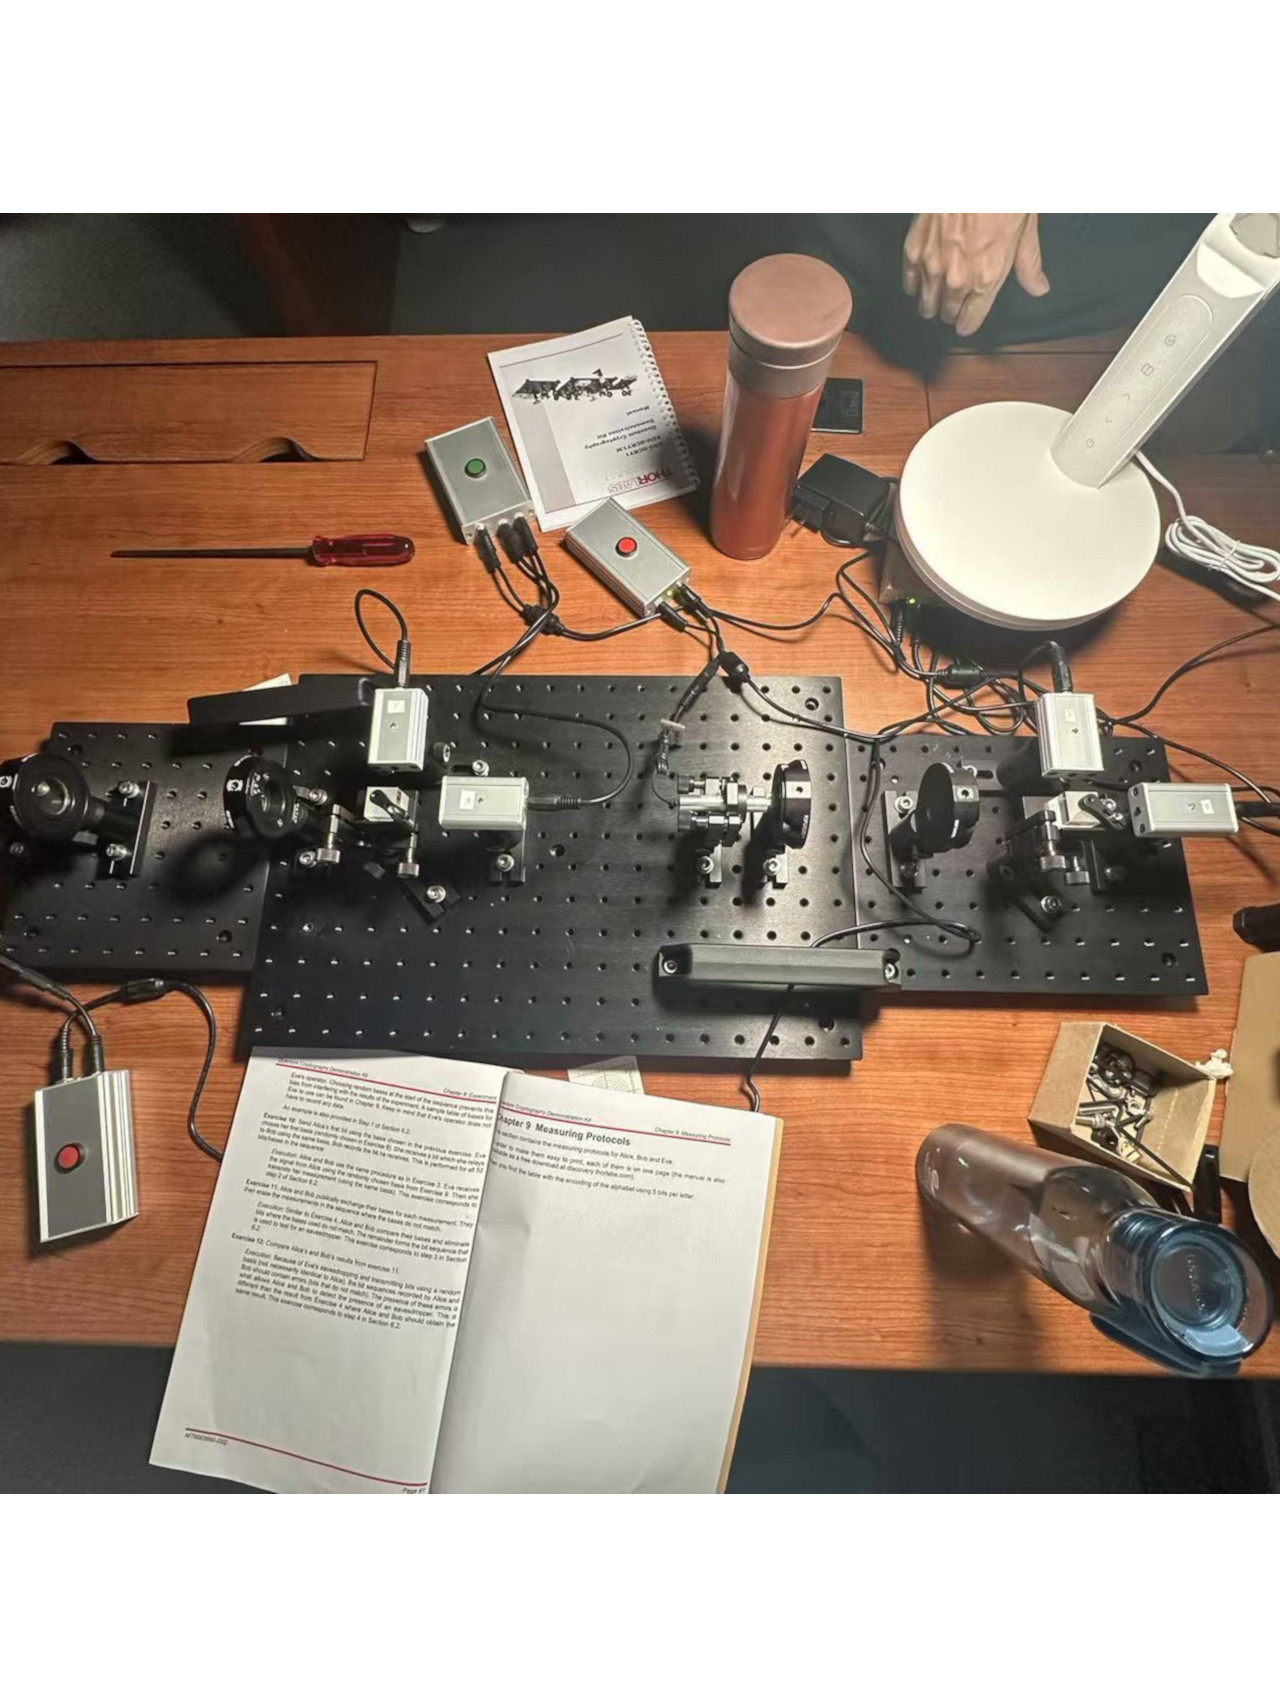
\includegraphics[width=0.2\textwidth,height=0.3\textwidth]{pictures/微信图片_20241031162855.jpg}
    \caption{包含 Bob, Eve, Alice 的完整实验系统}
\end{figure}

\subsection{密钥生成实验}
先将实验平台中的 Eve 部分移除,重新校对好 Alice 和 Bob,确保对于 Alice 发射的四种可能偏振与 Bob 测量偏振的两种可能基底的任意组合均能得到正确结果。

\begin{figure}[htbp]
    \centering
    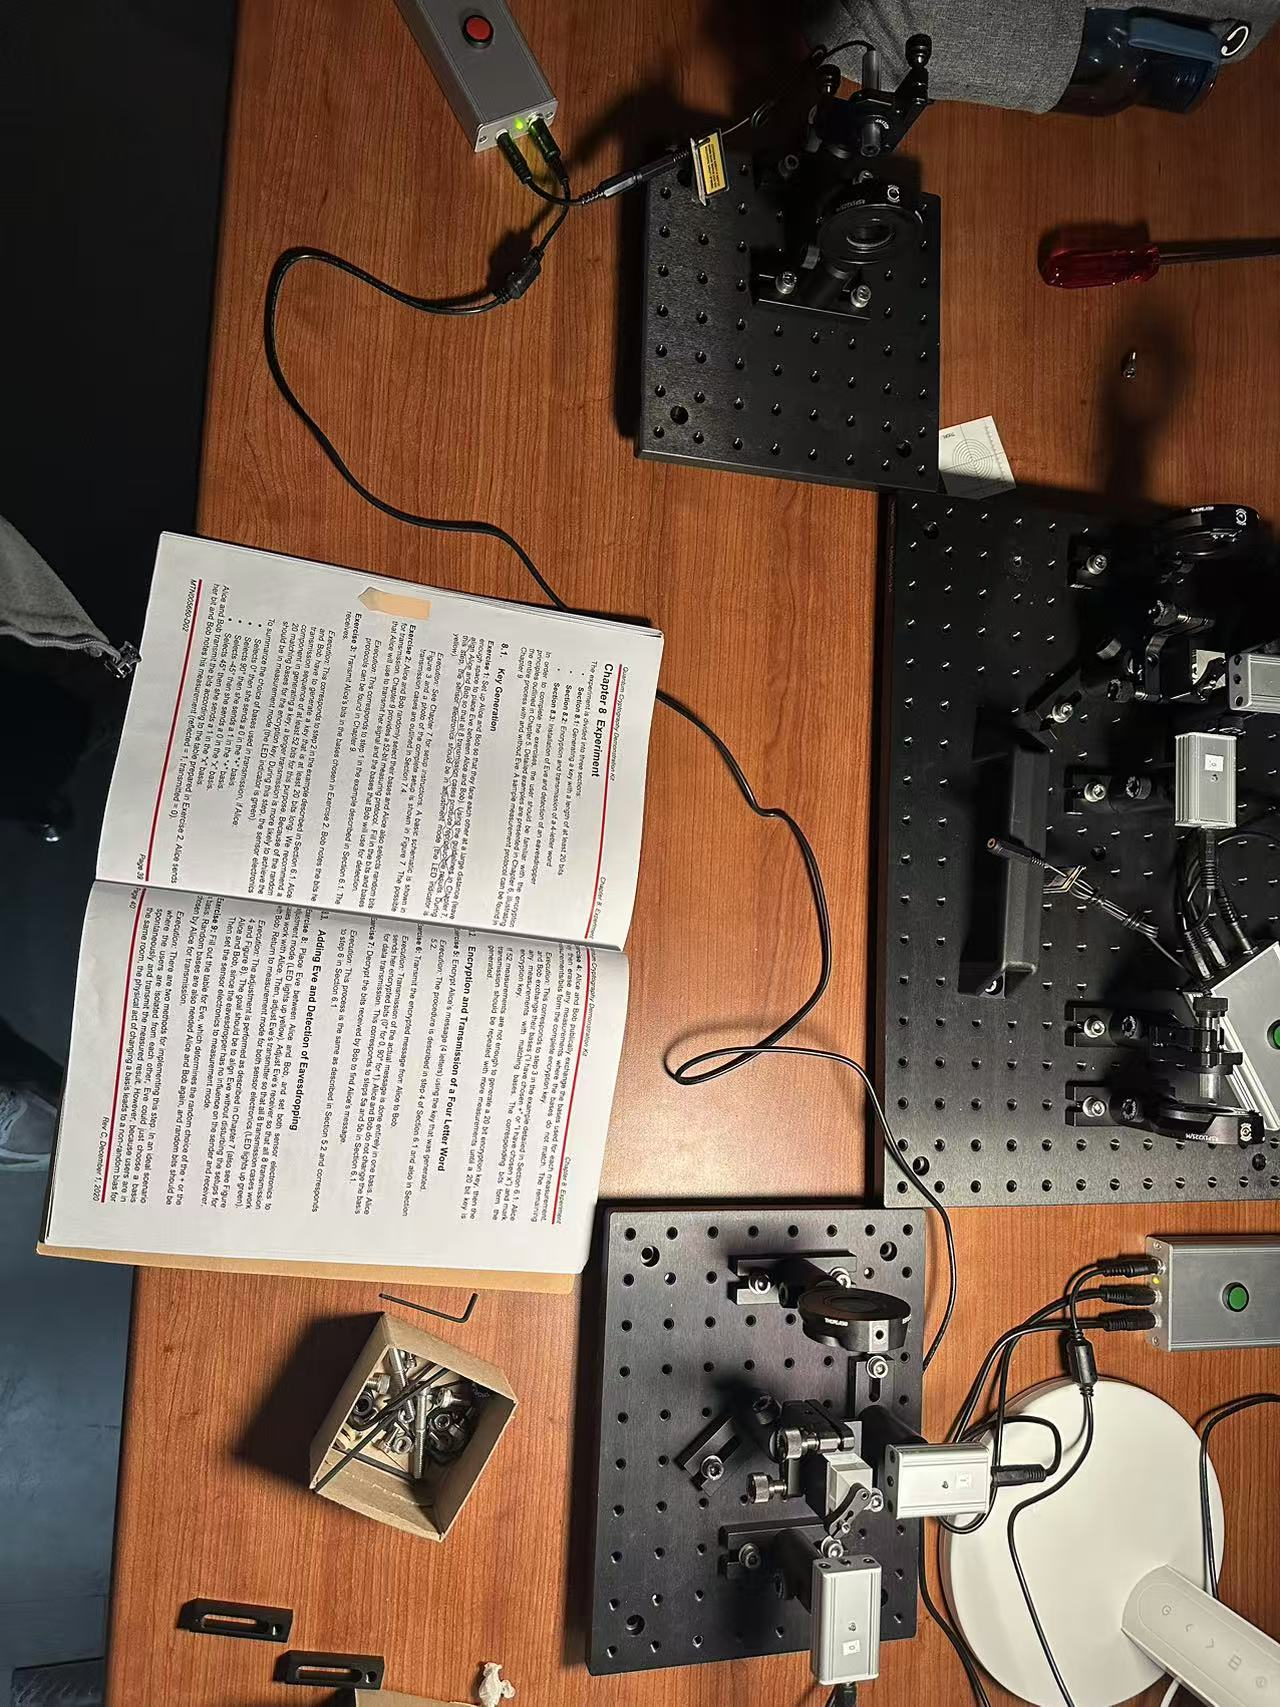
\includegraphics[width=0.2\textwidth,height=0.3\textwidth]{pictures/微信图片_20241031162758.jpg}
    \caption{仅包含 Bob, Alice 的实验系统}
\end{figure}

Alice 生成两段 52 bits 的随机基底和密钥,Bob 生成一段 52 bits 的随机基底。
\begin{lstlisting}[language=Python,numbers=left,caption=生成随机基底和密钥代码]
import random
AliceBase=AliceKey=BobBase=""
for i in range(52):
    AliceBase+=random.choice(['+','x'])
    AliceKey+=random.choice(['0','1'])
    BobBase+=random.choice(['+','x'])
\end{lstlisting}
\begin{lstlisting}
Alice Base: x+x++xxx+x++++xx+x+xxx+x++x++++++x+x+xxx+xx++xxx++xx
Alice Key:  1100010010100100010101001111101101101100110011000011
    
Bob Base:   xx++++x++x++x+++xx+x+x++++x++xxxx+xx++xx+x+x+++++x+x
\end{lstlisting}

Alice 用其选择的基底发送其生成的密钥,Bob 用自己选择的基底测量收到的光子。以下是 Bob 收到的光子的测量结果:
\begin{lstlisting}
Bob Receive:1110000010100111010111001111101110001100110010010111
\end{lstlisting}

Alice 和 Bob 交换各自随机选择的基底,去除使用不同基底的位,保留使用相同基底的测量结果作为密钥。
\begin{lstlisting}[language=Python,numbers=left,caption=求得最终密钥代码]
    AliceEncryptKey=BobEncryptKey=""
    for i in range(52):
        if AliceBase[i]==BobBase[i]:
            AliceEncryptKey+=AliceKey[i]
            BobEncryptKey+=BobReceive[i]
\end{lstlisting}
\begin{lstlisting}
Alice Encrypt Key: 1000101011011011111010011101

Bob Encrypt Key:   1000101011011011111010011101
\end{lstlisting}

此时 Alice 和 Bob 都得到了长度为 28 bits 的相同的密钥。他们接下来将用这组密钥加密并传输数据。

Alice 想传输的信息为 FENG,他先根据英文字母和二进制比特的对应表将信息转为 20 bits 待传输数据,接着用上面得到的密钥加密。
\begin{lstlisting}
Data:      00101001000110100110
EncryptKey:1000101011011011111010011101
Encrypted: 10100011110000011000
\end{lstlisting}

Alice 和 Bob 均采用 + 作为基底,Alice 将加密后的密文用 + 基底发给 Bob,Bob 接收测量后用自己的密钥解密得到原始数据。
\begin{lstlisting}
BobReceive:10100011110000011000
EncryptKey:1000101011011011111010011101
Data:      00101001000110100110
\end{lstlisting}

查询字母二进制对应表,可以还原出传递信息为 FENG。这样,Alice 和 Bob 成功利用量子分发的密钥加密传输了四个字母。

\subsection{窃听检测实验}
\begin{enumerate}
\item 在光路中加入Eve的测量装置
\begin{figure}[htbp]
    \centering
    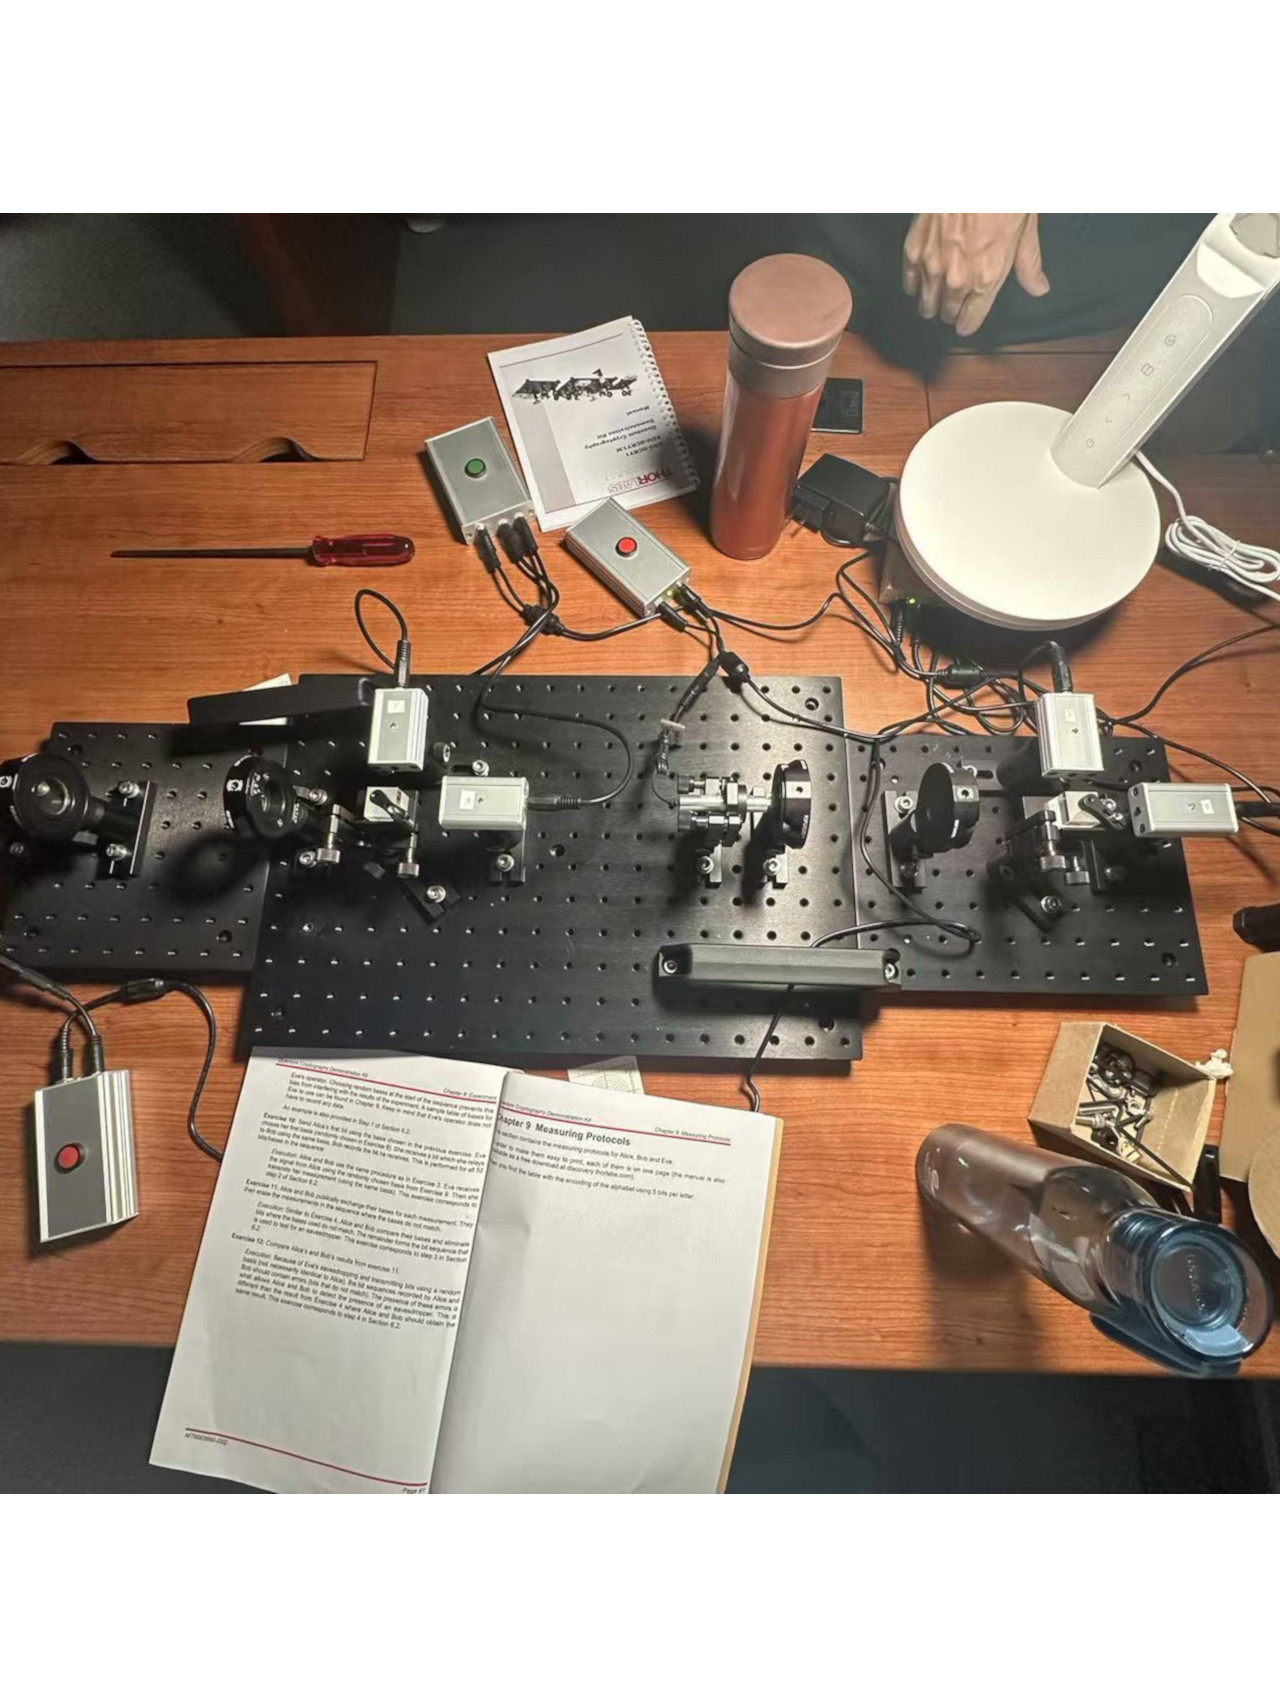
\includegraphics[width=0.2\textwidth,height=0.3\textwidth]{pictures/微信图片_20241031162855.jpg}
    \caption{包含 Bob, Eve, Alice 的完整实验系统}
\end{figure}
\item Alice,Bob和Eve各自随机选一对基,Alice选择要发送的信息
\begin{lstlisting}
    Alice Base: x+++x+x+++xxxxx++x+xx++++x++x+x+++x++x+x+xxxxxxx+++x
    Alice Key:  0011100010101000001111110001000010101101011100110010
    
    Bob Base:   x++x+++x+xx+xxx++x+xxxxx++xx+x+xxx+++x+++++++xxx+++x

    Eve Base:   x++x+++++x+x++x++++xx+x+++xxx++++x++++xx+xxx++x+x+++
\end{lstlisting}


\item 进行传输过程

Alice和Bob基于各自的基底传输数据,但是由于Eve在中间用他的基(0或45度)窃听,所以只有在Eve的基和Alice相同时Bob才能收到正确的信息,如果基底不同,Bob收到的信息将是随机的。

\begin{lstlisting}
    Bob Base:x++x+++x+xx+xxx++x+xxxxx++xx+x+xxx+++x+++++++xxx+++x
    Bob Rece:0010100111000100011110000000110101101001001001100011
\end{lstlisting}
\item 结果分析

经过比较(代码如下)
\begin{lstlisting}[language=python]
def compare_strings(str1, str2):
    differences = []
    for i in range(min(len(str1), len(str2))):
        if str1[i] == str2[i]:
            differences.append((i, str1[i], str2[i]))
    return differences

differences = compare_strings(AliceBase, Bob)
print(differences)
same_positions = ''.join([AliceMessage[i] for i, _, _ in differences])
print(same_positions)
\end{lstlisting}
结果得到,在Alice和Bob基相同的位置,
\begin{lstlisting}
A发出的Bit:    0010111000001110011000110010
Bob收到的Bit:  0010100100011110010001100011
\end{lstlisting}

比较得到,相同基一共有28Bit,其中有8Bit是错误的,错误率约为28\%,与理论预测的25\%相符。
\end{enumerate}
\section{实验思考}
\begin{enumerate}
\item 本实验使用的是脉冲激光而非单光子源,这与实际的量子密码系统有何区别?
\item BB84协议中为什么要使用两组不同的基底?
\item 在有窃听者的情况下,为什么会出现约25\%的错误率?
\item 量子密码学相比经典密码学有哪些优势和局限性?
\end{enumerate}

\section{总结}
\begin{itemize}
\item 通过实验成功演示了BB84量子密钥分发协议的工作原理
\item 验证了窃听检测机制的有效性
\item 理解了量子密码学中的关键概念如基底选择、量子测量等
\item 掌握了量子通信系统的基本组成和调试方法
\end{itemize}

\end{document}